% Created 2020-05-20 Wed 13:52
% Intended LaTeX compiler: pdflatex
\documentclass[11pt]{article}
\usepackage[utf8]{inputenc}
\usepackage[T1]{fontenc}
\usepackage{graphicx}
\usepackage{grffile}
\usepackage{longtable}
\usepackage{wrapfig}
\usepackage{rotating}
\usepackage[normalem]{ulem}
\usepackage{amsmath}
\usepackage{textcomp}
\usepackage{amssymb}
\usepackage{capt-of}
\usepackage{hyperref}
\usepackage{minted}
\usepackage[a4paper,margin=20mm]{geometry}
\usepackage{amsmath}
\usepackage{amsfonts}
\usepackage{stmaryrd}
\usepackage{bm}
\usepackage{minted}
\usemintedstyle{emacs}
\usepackage[T1]{fontenc}
\usepackage[scaled]{beraserif}
\usepackage[scaled]{berasans}
\usepackage[scaled]{beramono}
\newcommand{\tr}{\textsf{T}}
\newcommand{\grad}{\bm{\nabla}}
\newcommand{\av}[2][]{\mathbb{E}_{#1\!}\left[ #2 \right]}
\newcommand{\Prob}[2][]{\mathbb{P}_{#1\!}\left[ #2 \right]}
\newcommand{\logg}[1]{\log\!\left( #1 \right)}
\newcommand{\pred}[1]{\left\llbracket { \small #1} \right\rrbracket}
\newcommand{\e}[1]{{\rm e}^{#1}}
\newcommand{\dd}{\mathrm{d}}
\newcommand{\ii}{\mathrm{i}}
\DeclareMathAlphabet{\mat}{OT1}{cmss}{bx}{n}
\newcommand{\normal}[2]{\mathcal{N}\!\left(#1 \big| #2 \right)}
\newcounter{eqCounter}
\setcounter{eqCounter}{0}
\newcommand{\explanation}{\setcounter{eqCounter}{0}\renewcommand{\labelenumi}{(\arabic{enumi})}}
\newcommand{\eq}[1][=]{\stepcounter{eqCounter}\stackrel{\text{\tiny(\arabic{eqCounter})}}{#1}}
\newcommand{\argmax}{\mathop{\mathrm{argmax}}}
\newcommand{\Dist}[2][Binom]{\mathrm{#1}\left( \strut {#2} \right)}
\newcommand{\goesto}[1]{\stackrel{#1}{\longrightarrow}}
\author{Adam Prügel-Bennett}
\date{\today}
\title{Computational Biology Subsidary Notes\\\medskip
\large Lecture 17: Dynamical Systems}
\hypersetup{
 pdfauthor={Adam Prügel-Bennett},
 pdftitle={Computational Biology Subsidary Notes},
 pdfkeywords={},
 pdfsubject={},
 pdfcreator={Emacs 26.3 (Org mode 9.1.9)}, 
 pdflang={English}}
\begin{document}

\maketitle

\section{Keywords}
\label{sec:org3176690}
\begin{itemize}
\item ODEs, nullclines, fixed points, stability analysis, bifications
\end{itemize}

\section{Main Points}
\label{sec:orgc1a9626}

\subsection{Understanding ODEs}
\label{sec:org0c4dff3}
\begin{itemize}
\item Understanding systems of ODEs is a classic problem in what is
known as \emph{dynamical systems}
\item To save on notation I'm going to drop writing concentrations of
\(X\) as \([X]\) (this is just me being lazy)
\item I am going to use examples to illustrate dynamics rather
concentrate on biology, although you can try to imagine a
scenario where the dynamics describes some biological process
\item The type of equations I am considering are a set of equations for
variables (molecular species) \(\bm{X}=(X_1,X_2,\ldots,X_n)\)
governed by
\[ \frac{\dd X_i}{\dd t} = f_i(\bm{X}) \]
\begin{itemize}
\item \(f_i(\bm{X})\) describes a set of terms that potentially depends
on the concentrations all the other species
\end{itemize}
\end{itemize}
\subsubsection{Two Species}
\label{sec:org2d15961}
\begin{itemize}
\item We consider a system where \(X_2\) acts as a repressor
for the production of \(X_1\) and \(X_1\) turns into \(X_2\)
\begin{align*}
\varnothing &\goesto{f(X_2)} X_1 &
X_1 &\goesto{k_3} \varnothing & X_1 &\goesto{k_5} X_2 \\
\varnothing &\goesto{k_2} X_2 & X_2 &\goesto{k_4} \varnothing &&
\end{align*}
with
\[ f(X_2) &= \frac{k_1}{1+(X_2/K)^n} \]
\item The ODE describing these species are
\begin{align*}
 \frac{\dd X_1(t)}{\dd t} &= \frac{k_1}{1+(X_2(t)/K)^n} - k_3 \,
                          X_1(t)- k_5\,X_1(t) \\
\frac{\dd X_2(t)}{\dd t} &= k_2 + k_5\,X_1(t) - k_4\,X_2(t)
\end{align*}
\item To solve the ODE we need to provide some initial conditions
\item In Figure \ref{fig:coupledODE} we show the dynamics assuming
\(X_1=X_2=0\) and with parameter values of \(K=1\), \(k_1=20\),
\(k_2=k_3=k_4=5\), \(k_5=2\) and \(n=4\)
\begin{figure}[htbp]
\centering
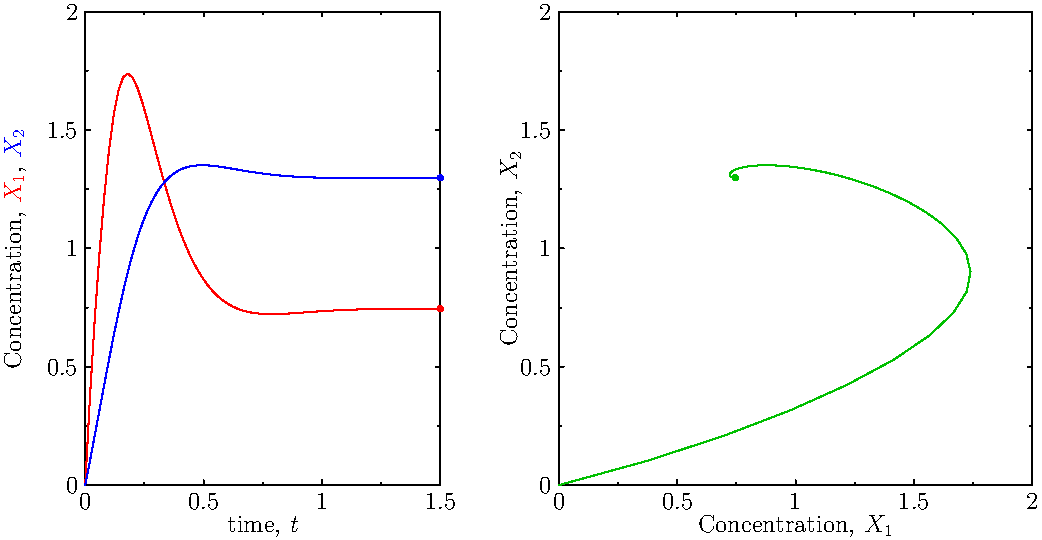
\includegraphics[width=0.6\textwidth]{./figures/coupledODE-41.pdf}
\caption{Dynamics for two interaction species \label{fig:coupledODE}}
\end{figure}
\item However, it is useful to understand the dynamics from any
initial conditions
\item In Figure \ref{fig:trajectories} we show some trajectories
starting from different initial points as well as the vector
field of derivatives (flow fields shown as arrows)
\begin{figure}[htbp]
\centering
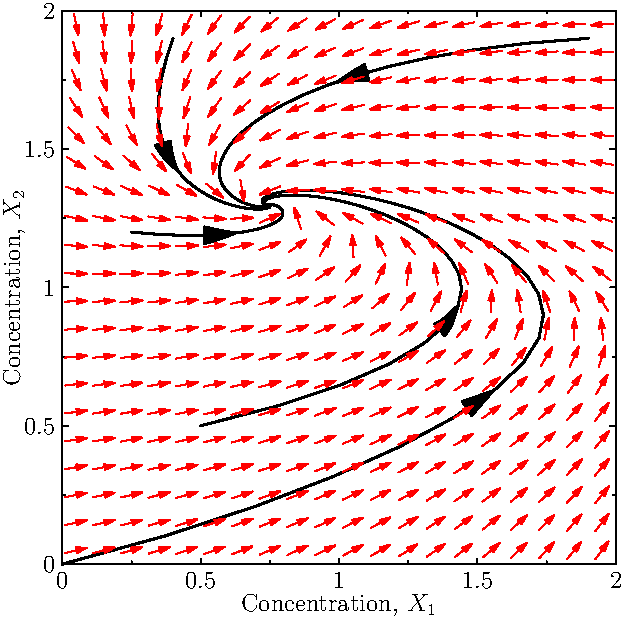
\includegraphics[width=0.35\textwidth]{./figures/trajectories-1.pdf}
\caption{Trajectory and flow field for two species system \label{fig:trajectories}}
\end{figure}
\item To get a better analytic understanding of what is going on we
can compute the \textbf{nullclines}: these are curves where
\({\displaystyle \tfrac{\dd X_i}{\dd t} =0}\)
\item For this system
\begin{align*}
\frac{\dd X_1}{\dd t} &= \frac{k_1}{1+(X_2/K)^n} - k_3 \,
                         X_1- k_5\,X_1 = 0
      & &\Rightarrow &
X_1 &= \frac{k_1}{(k_3+k_5)(1+(X_2/K)^n)}
      \\ \\
\frac{\dd X_2}{\dd t} &= k_2 + k_5\,X_1 - k_4\,X_2=0
      &&\Rightarrow &
X_2 &= \frac{k_2 + k_5\,X_1}{k_2}
\end{align*}
\item Where the nullclines intersect we have a \emph{stationary point}
\item We plot the nullclines in Figure \ref{fig:nullclines}
\begin{figure}[htbp]
\centering
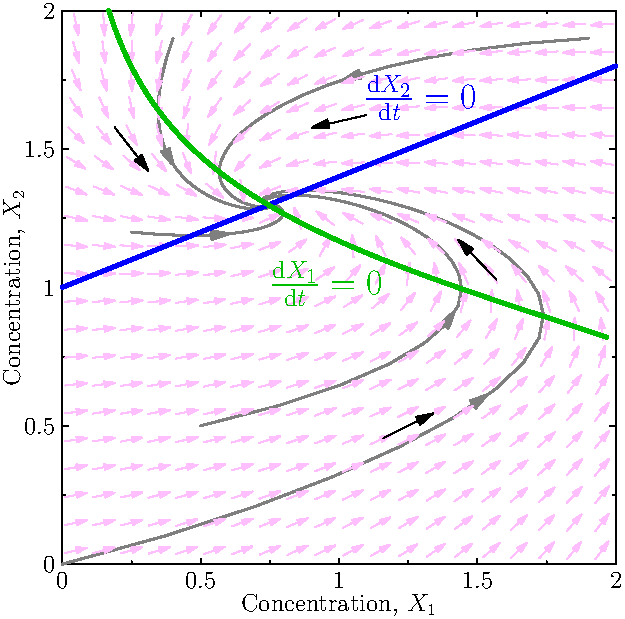
\includegraphics[width=0.35\textwidth]{./figures/nullclines-3.pdf}
\caption{Nullclines for two species system \label{fig:nullclines}}
\end{figure}
\end{itemize}

\subsection{Stability}
\label{sec:orge861d5b}
\begin{itemize}
\item Having identified fixed points (where nullclines intersect) we
investigate their stability
\item Let us consider a slightly different system
\item Here \(X_1\) and \(X_2\) are proteins that inhibit each other's
expression
\begin{align*}
  \frac{\dd X_1(t)}{\dd t} &= \frac{k_1}{1+(X_2(t)/K_2)^{n_1}} - k_3 \, X_1(t)\\
  \frac{\dd X_2(t)}{\dd t} &= \frac{k_2}{1+(X_1(t)/K_1)^{n_2}} - k_4\,X_2(t)
\end{align*}
\item If we consider the symmetric case \(k_1=k_2=20\), \(K_1=K_2=1\),
\(k_3=k_4=5\), \(n_1=n_2=4\) (later we explore changing the parameters)
\item We can again compute the flow fields and nullclines
\item These are shown in Figure \ref{fig:bistable}
\begin{figure}[htbp]
\centering
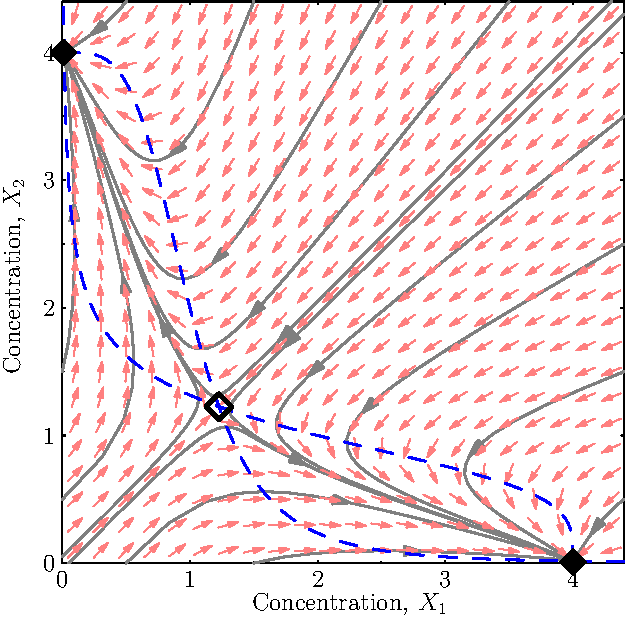
\includegraphics[width=0.35\textwidth]{./figures/bistable-4.pdf}
\caption{Nullclines and flow field for bistable system  \label{fig:bistable}}
\end{figure}
\item The nullclines intersect at three points leading to three fixed-point
\item The flow fields show that almost all trajectories flow either to
the fixed point with \(X_1\gg X_2\) or with \(X_2\gg X_1\)
\item There is a third unstable fixed point when \(X_1=X_2\) but this is
unstable to any perturbation that breaks the symmetry
\item Although it seems that we can investigate fixed-points
graphically, this only works in low dimensions (where we have a
few species) and doesn't give us insight on how the stability
depends on the parameters of the model
\end{itemize}

\subsubsection{Fixed-Point Analysis}
\label{sec:orga304e1a}
\begin{itemize}
\item As I said previously these systems are highly non-linear and it
is very unlikely that we can solve the dynamics in closed form
\item However, there is a very general procedure for understanding the
stability of fixed-points
\item We linearise the dynamics around the fixed point
\item Recall that we have a set of ODEs
\[ \frac{\dd X_i}{\dd t} = f_i(\bm{X}) \]
\item Now assume we are at a point \(\bm{X}=\bm{X}^{*}+\bm{\epsilon}\) where
\(\bm{X}^{*}\) is a fixed point
\item We can Taylor expand \(f_i(\bm{X})\) around \(\bm{X}^{*}\)
\begin{align*}
 \frac{\dd X_i}{\dd t} = f_i(\bm{X}^*+\bm{\epsilon})
 \approx f_i(\bm{X}^*) + \bm{\epsilon}^\tr \grad f_i(\bm{X}^*) + O(\bm{\epsilon}^2)
 = \bm{\epsilon}^\tr \grad f_i(\bm{X}^*) + O(\bm{\epsilon}^2)
\end{align*}
where we have used \(f_i(\bm{X}^*)=0\) as we are at a fixed point
\item Writing this in vector form
\begin{align*}
\frac{\dd \bm{X}}{\dd t} = \bm{f}(\bm{X}^*+\bm{\epsilon})
=  \mat{J}\, \bm{\epsilon} + O(\bm{\epsilon}^2)
 \end{align*}
\begin{itemize}
\item where \(\mat{J}\) is the \textbf{Jacobian} matrix with elements
\begin{align*}
  J_{ij} = \left. \frac{\partial f_i(\bm{X})}{\partial X_j}\right|_{\bm{X}=\bm{X}^*}
\end{align*}
\end{itemize}
\item Since \(\bm{\epsilon}(t) = \bm{X}(t) - \bm{X}^*\) then
\begin{align*}
  \frac{\dd \bm{\epsilon}(t)}{\dd t} = \frac{\dd \bm{X}(t)}{\dd t}
  \approx \mat{J}\, \bm{\epsilon}(t)
\end{align*}
\item To solve this we use the eigenvalue decomposition of \(\mat{J}\)
     \begin{align*}
  \mat{J} = \mat{V} \mat{\Lambda}\,\mat{V}^{-1}
\end{align*}
\begin{itemize}
\item Where \(\mat{\Lambda}\) is a diagonal matrix whose elements
\(\Lambda_{ii}=\lambda_i\) are eigenvalues of \(\mat{J}\) and the
columns of \(\mat{V}\) are the eigenvectors
\item For non-symmetric matrices (such as \(\mat{J}\) usually) the eigenvalues
are either real or appear in pairs, \(\lambda_i\) and
\(\lambda_{i+1}\) where \(\lambda_{i+1} = \lambda_i^{*}\) (i.e. they
are complex conjugate pairs
\item In this case the corresponding eigenvectors \(\bm{v}_i\) and
\(\bm{v}_{i+1}\) will also occur in complex conjugate pairs
\(\bm{v}_{i+1}=\bm{v}_i^{*}\)
\item Thus
\begin{align*}
\frac{\dd \bm{\epsilon}(t)}{\dd t}
 &= \mat{V} \mat{\Lambda}\,\mat{V}^{-1}\, \bm{\epsilon}(t)
 &\Rightarrow&&
 \frac{\dd \mat{V}^{-1}\bm{\epsilon}(t)}{\dd t} 
 &\approx \mat{\Lambda}\, \mat{V}^{-1}\bm{\epsilon}(t)
\end{align*}
where we multiply both sides by \(\mat{V}^{-1}\)
\item Defining \(\hat{\bm{\epsilon}}(t) = \mat{V}^{-1}\bm{\epsilon}(t)\) then
\begin{align*}
 \frac{\dd \hat{\bm{\epsilon}}(t)}{\dd t} 
  &\approx \mat{\Lambda}\, \hat{\bm{\epsilon}}(t) & &\text{or} &
  \frac{\dd \hat{\epsilon}_i(t)}{\dd t} 
  &\approx \lambda_i\, \hat{\epsilon_i}(t)\pause
\end{align*}
\item This aligns the perturbations with the eigenvectors of \(\mat{J}\)
\item We can solve these equations giving
\[ \hat{\epsilon}_i(t) \approx \e{\lambda_i\,t}\,  \,\hat{\epsilon}_i(0) \]
\begin{itemize}
\item If \(\lambda_i\) is real and positive the any
perturbation in the direction \(\bm{v}_i\) will grow with time
\item If \(\lambda_i\) is real and negative then any
perturbation in the direction \(\bm{v}_i\) will shrink
\item If \(\lambda_i\) and \(\lambda_{i+1}\) are complex conjugate
pairs then the  trajectory in the plane spanned by \(\bm{v}_i\)
and \(\bm{v}_{i+1}\) will be a spiral around the fixed-point
\begin{itemize}
\item It will spiral out if the real part of the eigenvalues
are positive and spiral in if the real values of
the eigenvalues are negative
\end{itemize}
\end{itemize}
\item The fixed point is stable if \textbf{all} eigenvalues satisfy \(\Re\, \lambda_i<0\)
\end{itemize}
\item For the bistable system, the unstable fixed point is at \(X_1=X_2=1.226\)
\item The Jacobian is
\[ \mat{J} = \begin{pmatrix}
        -5 & -13.87 \\
         -13.87 & -5
      \end{pmatrix} \]
 This has eigenvalues are 8.868 and \(-18.868\) in the directions
 \(\binom{1}{-1}\) and \(\binom{1}{1}\), respectively.  Clearly
 this is unstable to perturbations that break the symmetry
 between \(X_1\) and \(X_2\).
\item \textbf{Oscillator}
\begin{itemize}
\item We consider the process of generating \(X_2\) through an
intermediary \(X_1\) where the production of \(X_2\) from \(X_1\) is
catalysed by the presence of \(X_2\)
\begin{align*}
\varnothing &\goesto{k_0} X_1 &
X_1 &\goesto{f(X_2)} X_2 &
X_2 &\goesto{k_2} \varnothing
\end{align*}
where \(f(X_2) = k_1\left(1+ (X_2/K)^n\right)\)
\item This leads to the coupled pair of ODEs
\begin{align*}
 \frac{\dd X_1(t)}{\dd t} &= k_0 -
 k_1\,\left(1+\left(\frac{X_2(t)}{K}\right)^n\right)\,X_1(t) \\
 \frac{\dd X_2(t)}{\dd t} &=
  k_1\,\left(1+\left(\frac{X_2(t)}{K}\right)^n\right)\,X_1(t) -k_2\,X_2(t)
 \end{align*}
\item In Figure \ref{fig:oscillator} we show the dynamics for \(k_0=8\), \(k_1=1\), \(K=1\), \(k_2=5\) and \(n=2\)
\begin{figure}[htbp]
\centering
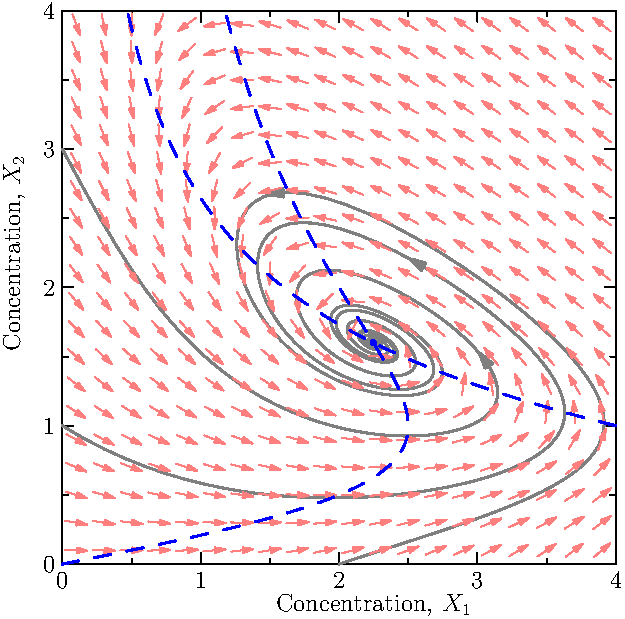
\includegraphics[width=0.35\textwidth]{./figures/oscillation-2.pdf}
\caption{Dynamics of Oscillator \label{fig:oscillator}}
\end{figure}
\item The fixed-point is given by
$$ \bm{X}^* = \left(\frac{k_0}{k_1(1+(k_0/(K\,k_2))^n)},
       \frac{k_0}{k_2}\right) = \left(\frac{200}{89},
       \frac{8}{5}\right) $$
\item The Jacobian is given by
\begin{align*}
 \mat{J}=
 \begin{pmatrix}
  -k_1\,\left(1+\left(\frac{X_2^*}{K}\right)^n\right) & 
- \frac{n\, k_1}{K}\,\left(\frac{X_2^*}{K}\right)^{n-1}\,X_1^* \\
 k_1\,\left(1+\left(\frac{X_2^*}{K}\right)^n\right) & 
 \frac{n\, k_1}{K}\,\left(\frac{X_2^*}{K}\right)^{n-1}\,X_1^* - k_2
\end{pmatrix} =
\begin{pmatrix}
\frac{-89}{25} & \frac{-640}{89}\\
\rule{0pt}{3ex} \frac{89}{25} & \frac{195}{89}
\end{pmatrix}
\end{align*}
\item Plugging this into Matlab (using \texttt{eig(J)})
\begin{align*}
\mat{J} =
\begin{pmatrix}
 \frac{-89}{25} & \frac{-640}{89}\\
 \rule{0pt}{3ex} \frac{89}{25} & \frac{195}{89}
\end{pmatrix}
= \mat{V}
\begin{pmatrix}
 -0.68 + 4.16\ii & 0 \\
 0  &  -0.68 - 4.16\ii
\end{pmatrix}
\mat{V}^{-1}
\end{align*}
where
\begin{align*}
\mat{V} = \begin{pmatrix}
 0.82 &   0.82 \\
 -0.33 - 0.47\ii  & -0.33 + 0.47\ii 
\end{pmatrix}
\end{align*}
\item The eigenvalues are \(-0.68 \pm 4.16\ii\) with eigenvectors of
\(\binom{0.82}{-0.33\pm0.47\ii}\)
\item Eigenvalues are a pain to compute by hand, but for \(2\times2\)
matrices we can compute them from the trace, \(T =
       \mathop{\mathrm{tr}} \mat{J} = J_{11} + J_{22}\), and determinant \(D=
       \det(\mat{J})=J_{11}\,J_{22}-J_{12}\,J_{21}\) where
$$ \lambda_{1,2} = T/2 \pm \sqrt{T^{2}/4-D} $$
\item The system is stable (the real part of the eigenvectors are
negative), but the  large complex component causes a
significant spiralling
\end{itemize}
\end{itemize}

\subsection{Bification}
\label{sec:org3f1e393}
\begin{itemize}
\item In understanding dynamical systems we can study how the fixed
points change as we vary the parameters of the system
\item Fixed points tend to appear in pairs, one stable and one unstable
\item Clearly if we have two stable fixed point then there will be some
manifold that divides the basins of attraction of the two fixed points
\item On this manifold there will usually exist an unstable fixed-point
\item To illustrate this we return to the bistable problem
\begin{align*}
 \frac{\dd X_1(t)}{\dd t} &= \frac{k_1}{1+(X_2(t)/K_2)^{n_1}} - k_3 \, X_1(t)\\
 \frac{\dd X_2(t)}{\dd t} &= \frac{k_2}{1+(X_1(t)/K_1)^{n_2}} - k_4\,X_2(t)
\end{align*}
\item Earlier on we examine the symmetric case when \(k_1 = k_2=20\),
\(K_1=K_2=1\), \(k_3=k_4=5\), \(n_1=n_2=2\)
\item Now as we vary \(k_1\) from a very small value to large value we
change the nullcline associated with \(\tfrac{\dd X_1(t)}{\dd t}=0\)
\item For \(k_1<16\) there is only one crossing of the nullclines leading
to one fixed-point
\begin{figure}[htbp]
\centering
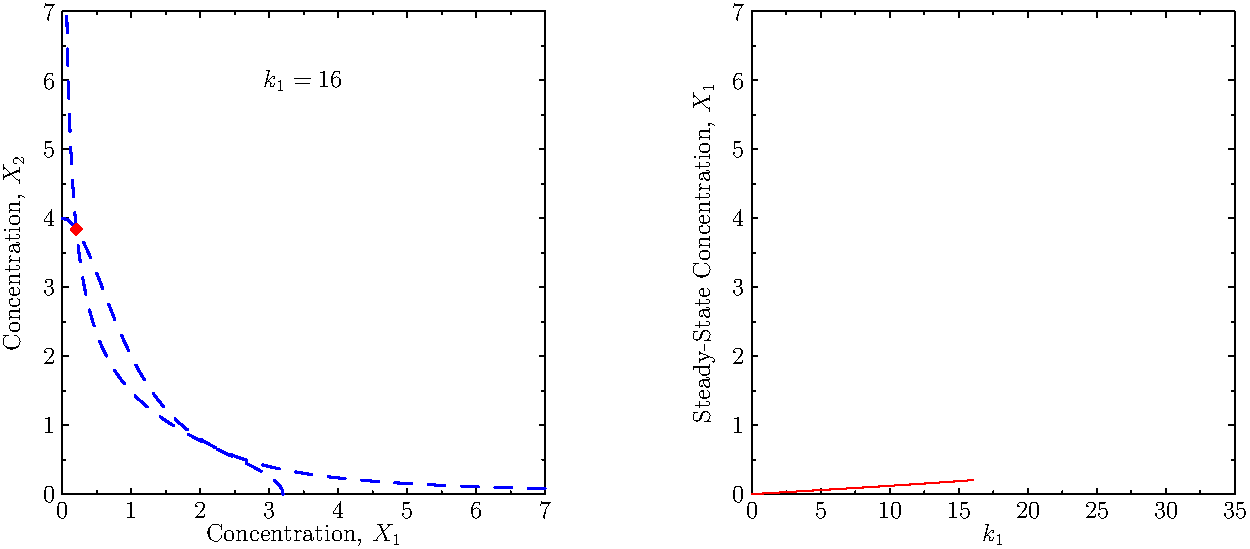
\includegraphics[width=0.6\textwidth]{./figures/bistableFP-13.pdf}
\caption{Dynamics of Oscillator \label{fig:oscillator}}
\end{figure}
\item Again for \(k_1>29\) there is only one fixed-point which persists
as we increase \(k_1\) further
\begin{figure}[htbp]
\centering
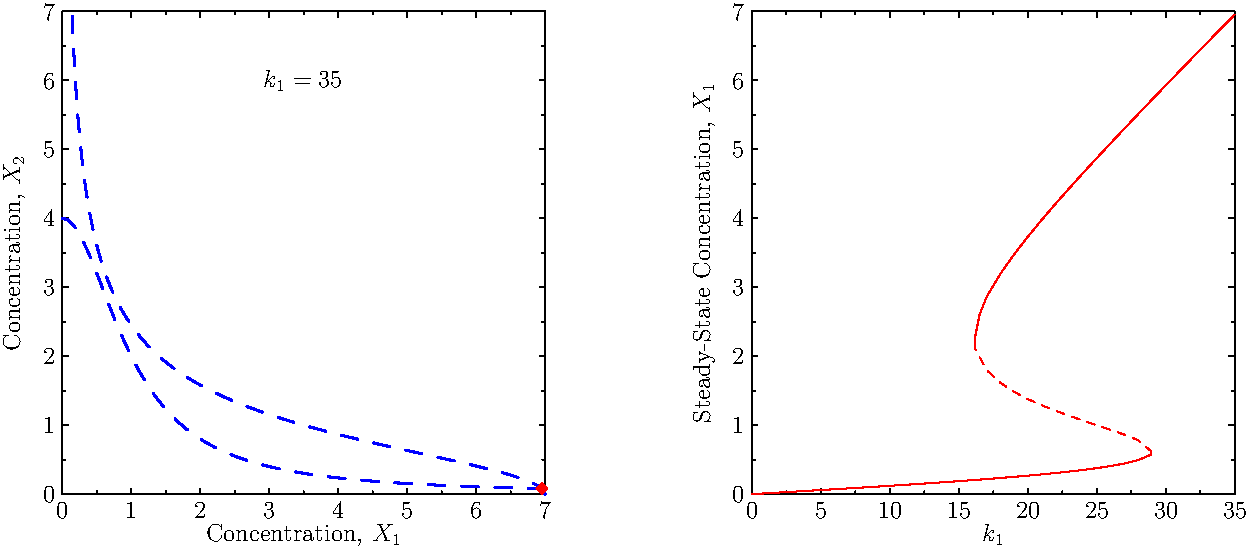
\includegraphics[width=0.6\textwidth]{./figures/bistableFP-32.pdf}
\caption{Dynamics of Oscillator \label{fig:oscillator}}
\end{figure}
\item The appearance of a pair of fixed-point is known as a \textbf{bification}
\item This type of behaviour can result in a \emph{hysteresis loop} where as you
change parameters you make a sudden jump when a stable
fixed-point annihilates with an unstable fixed-point.  Reversing
the change in the parameter you stay attracted to the second
fixed point.
\begin{figure}[htbp]
\centering
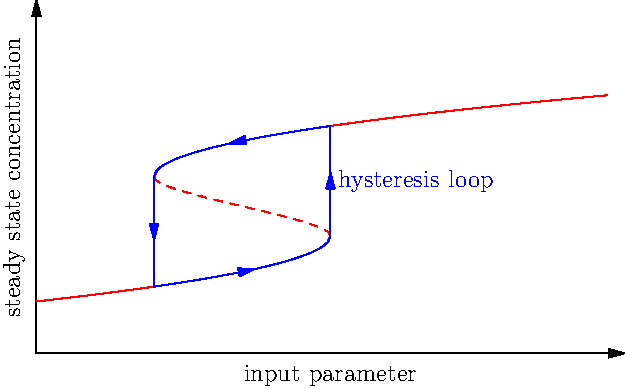
\includegraphics[width=0.4\textwidth]{./figures/hysteresis-52.pdf}
\caption{Dynamics of Oscillator \label{fig:oscillator}}
\end{figure}
\end{itemize}

\subsubsection{Hopf Bification}
\label{sec:orgb3a5b77}
\begin{itemize}
\item A second mechanism where the nature of the fixed-point changes
is when the stability of the fixed point changes
\item This happens in the autocatalytic reaction we looked at earlier
\begin{align*}
\frac{\dd X_1(t)}{\dd t} &= k_0 -
 k_1\,\left(1+\left(\frac{X_2(t)}{K}\right)^n\right)\,X_1(t) \\
\frac{\dd X_2(t)}{\dd t} &=
 k_1\,\left(1+\left(\frac{X_2(t)}{K}\right)^n\right)\,X_1(t) -k_2\,X_2(t)
\end{align*}
with \(k_0=8\), \(k_1=1\), \(K=1\), \(k_2=5\)
\item We consider what happens as we vary \(n\)
\begin{itemize}
\item For small \(n\) we have a stable fixed-point
\begin{figure}[htbp]
\centering
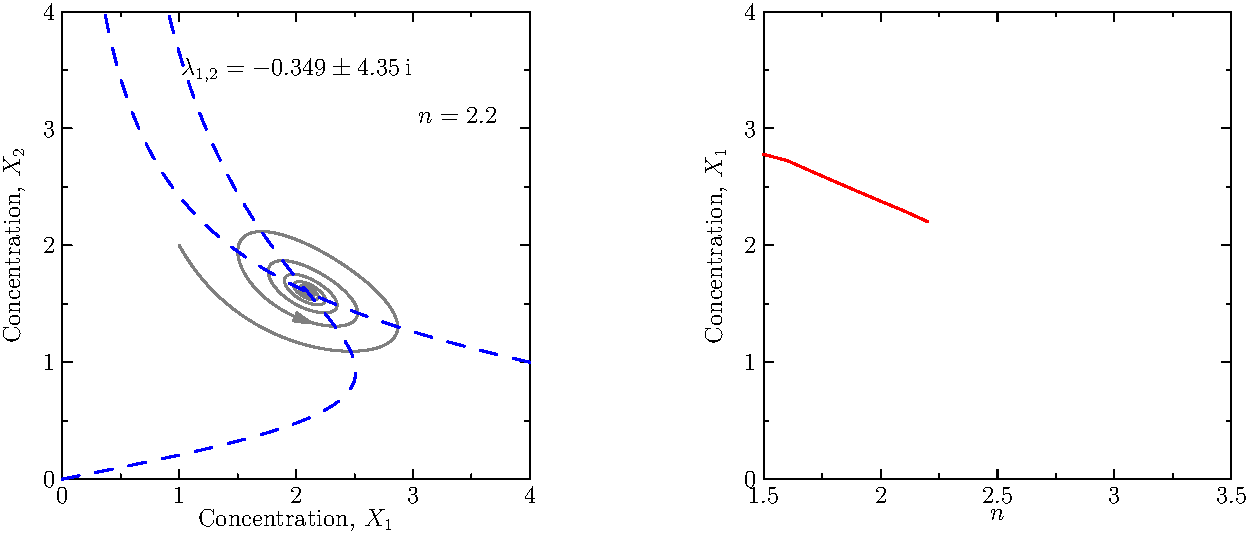
\includegraphics[width=0.6\textwidth]{./figures/hopfBif-7.pdf}
\caption{Dynamics of Oscillator \label{fig:oscillator}}
\end{figure}
\item As we increase \(n\) the fixed point becomes unstable
\begin{figure}[htbp]
\centering
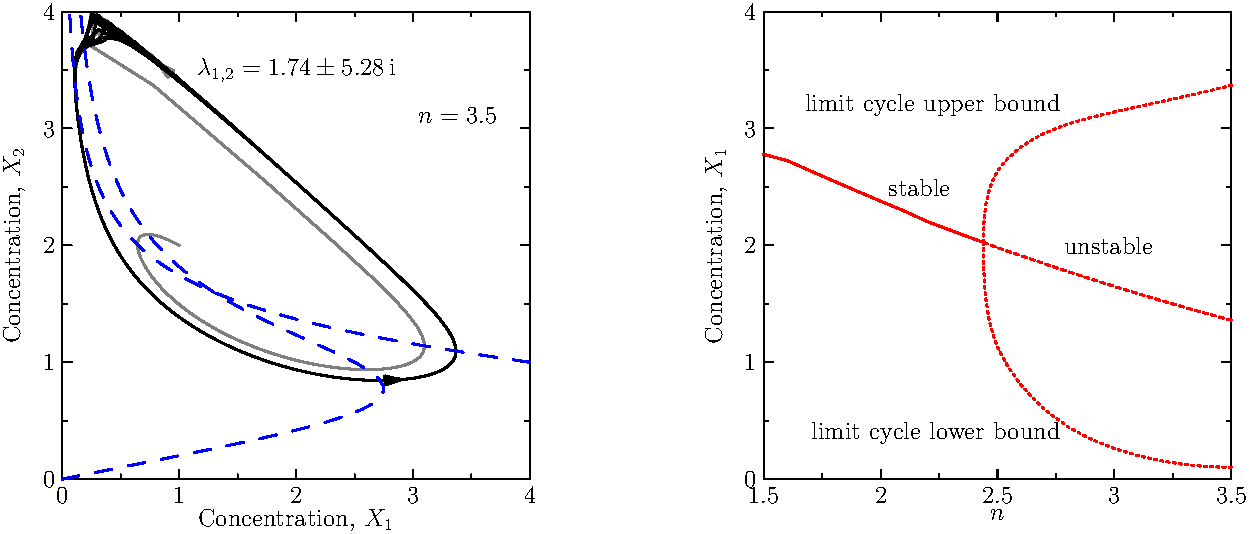
\includegraphics[width=0.6\textwidth]{./figures/hopfBif-21.pdf}
\caption{Dynamics of Oscillator \label{fig:oscillator}}
\end{figure}
\item In this case the dynamics converges to a \emph{limit cycle} that
oscillates around the unstable fixed point
\end{itemize}
\item This is known as a \emph{Hopf bification}
\end{itemize}
\end{document}
